%!LW recipe=pdflatex-shellescape
\documentclass[11pt]{article}

\usepackage{geometry}
\geometry{margin=0.5in}

\usepackage[utf8]{inputenc}
%\usepackage[english]{babel}

\usepackage{graphicx}
\usepackage[dvipsnames]{xcolor}
\usepackage{amsmath}
\usepackage{float}
\usepackage{natbib}
\bibliographystyle{mnras}
\setcitestyle{authoryear,open={(},close={)}}
%\usepackage[hybrid]{markdown}
\usepackage{enumitem}
\setitemize{itemsep=-2pt}
\usepackage[colorlinks=true,allcolors=blue]{hyperref}
\usepackage{caption}
\usepackage{overpic}

\begin{document}

\tableofcontents
\clearpage

\section{Description of the system}

\subsection{Theoretical considerations}

\begin{figure}
  \centering
  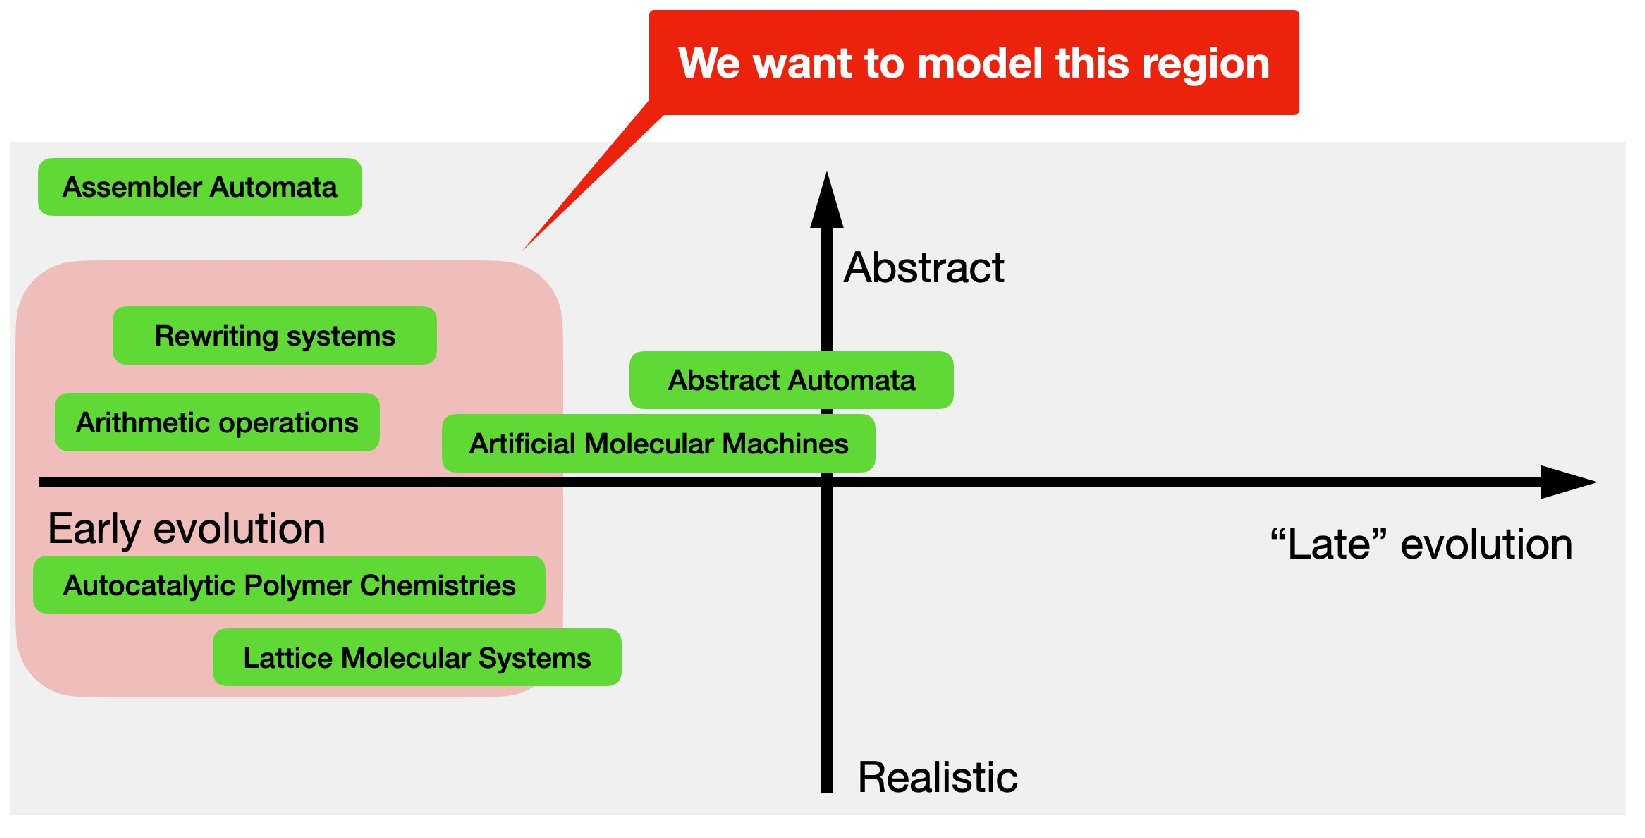
\includegraphics[width=0.75\textwidth]{figures/system/abstraction-stage.pdf}
  \caption{Classification of AC approaches along two axis: abstract vs realistic, and early vs late evolution. In the context of this project we will be focusing on the early evolution, using a balanced approach between more abstract and more realistic models.}
\end{figure}

\begin{figure}
  \centering
  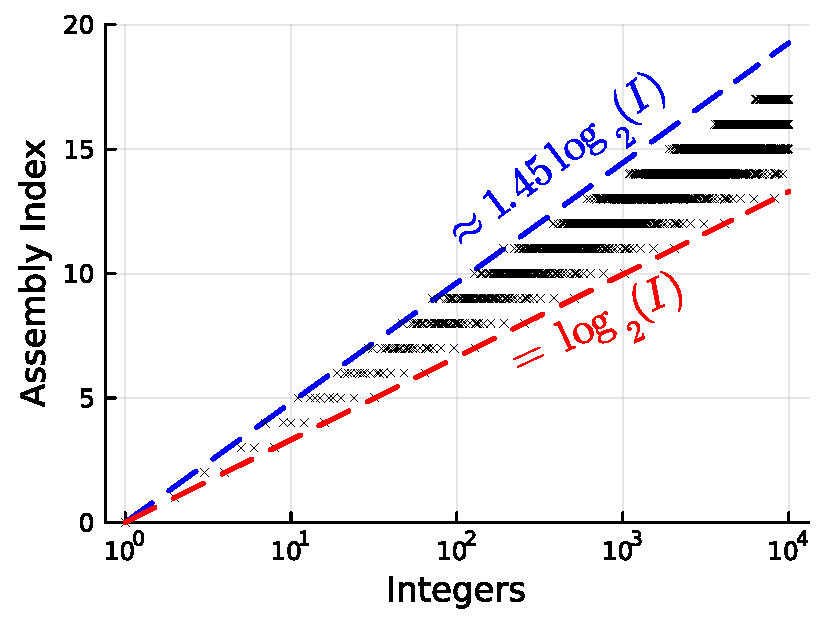
\includegraphics[width=0.50\textwidth]{figures/system/integers-assembly.pdf}
  \caption{...}
\end{figure}

\clearpage

\subsection{The model}

\begin{figure}
  \centering
  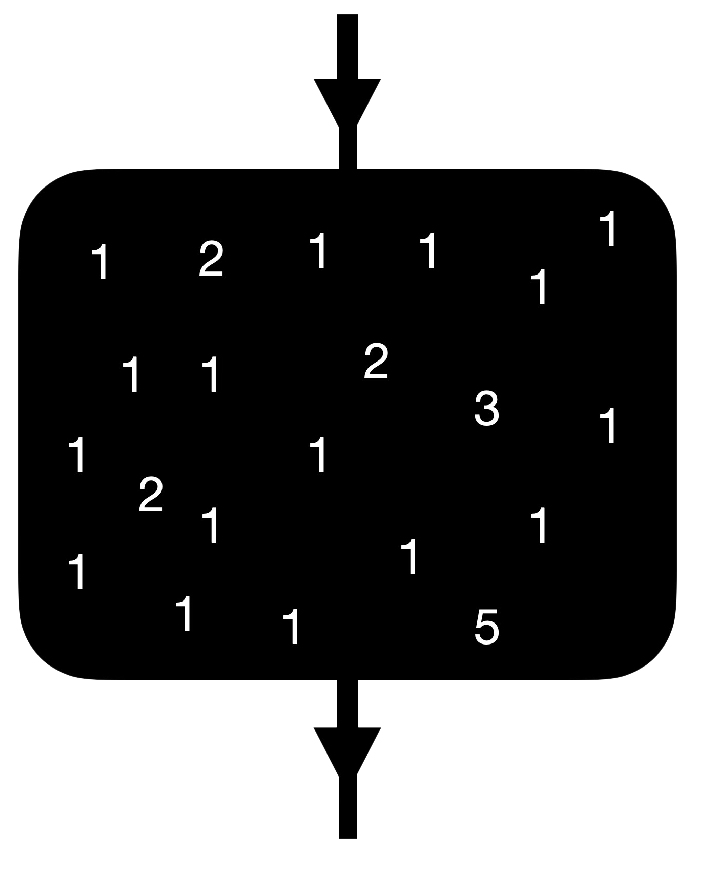
\includegraphics[width=0.35\textwidth]{figures/system/single-reactor.pdf}
  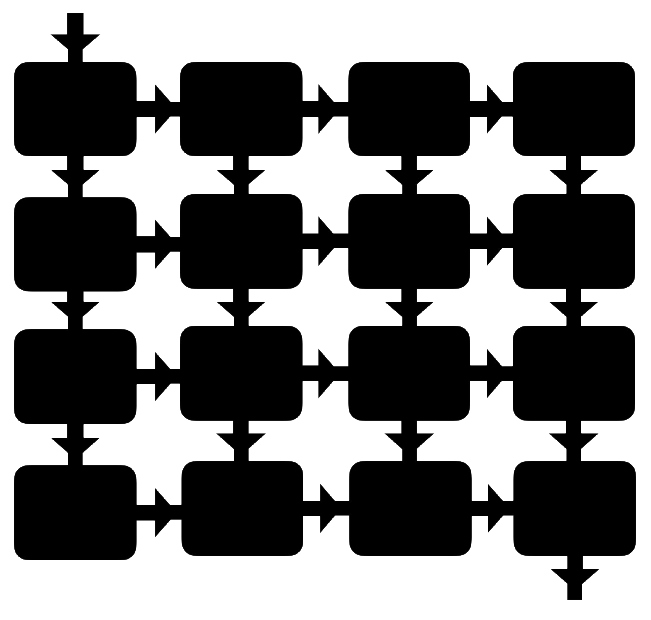
\includegraphics[width=0.45\textwidth]{figures/system/ensemble.pdf}
  \caption{single reactor + ensemble}
\end{figure}

\begin{figure}
  \centering
  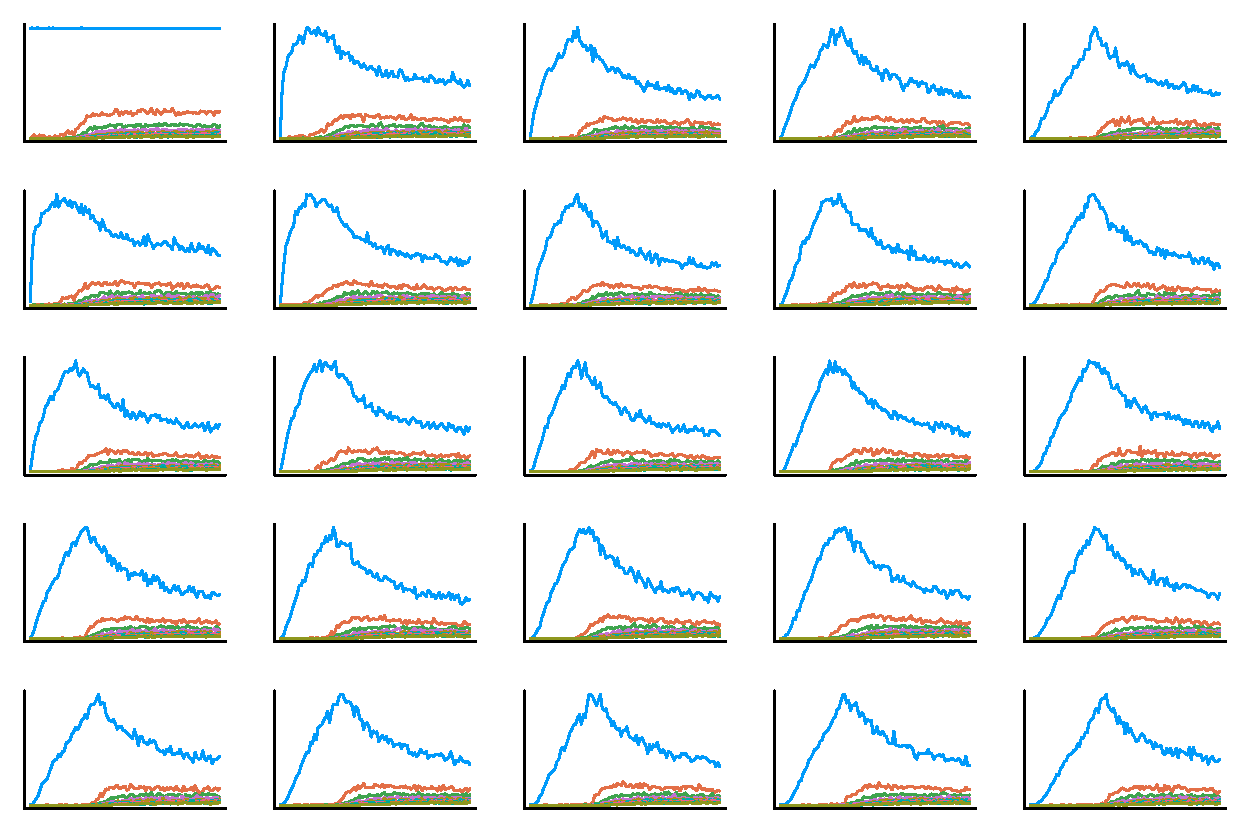
\includegraphics[width=0.75\textwidth]{figures/results/1-prelim/ts-gridplot.pdf}
  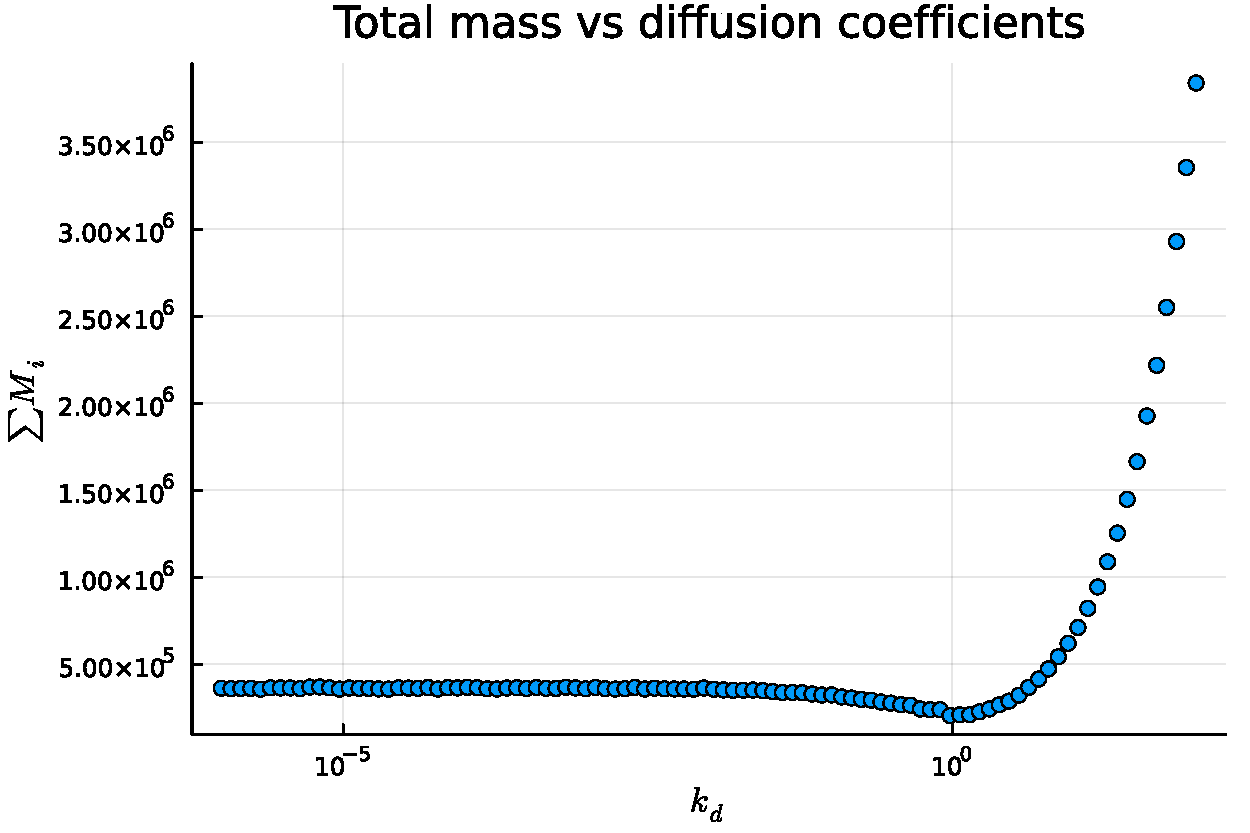
\includegraphics[width=0.50\textwidth]{figures/results/1-prelim/mass.pdf}
  \caption{...}
  \label{fig:prelim-gridplot}
\end{figure}

\section{Experiments}

\subsection{Preliminary experiments}

\subsubsection{Varying the diffusion rate}

\textit{Experiments performed in October 2024.}\\

Basically what we’ve done so far is vary the diffusion rate, plot the populations of chemical species across chemostats, and examine how the complexity varies when we change the diffusion. Here’s a few results (Fig.~\ref{fig:prelim})

\begin{figure}
  \centering
  \begin{overpic}[width=0.45\textwidth]{figures/results/1-prelim/mu-vs-kd.pdf}\put(-5,80){\textbf{(A)}}\end{overpic}
  \begin{overpic}[width=0.45\textwidth]{figures/results/1-prelim/sd-vs-kd.pdf}\put(-5,80){\textbf{(B)}}\end{overpic} \\
  \begin{overpic}[width=0.45\textwidth]{figures/results/1-prelim/abundance-I.pdf}\put(-5,70){\textbf{(C)}}\end{overpic}
  \begin{overpic}[width=0.45\textwidth]{figures/results/1-prelim/abundance-A.pdf}\put(-5,70){\textbf{(D)}}\end{overpic}
  \caption{\\\textbf{Panel (A)} shows ...\\ \textbf{Panel (B)} shows ...\\ \textbf{Panel (C)} shows ...\\ \textbf{Panel (D)} shows ...}
  \label{fig:prelim-diffusion}
\end{figure}

\begin{figure}
  \centering
  \begin{overpic}[width=0.45\textwidth]{figures/results/1-prelim/ensemble-distance.pdf}\put(-5,80){\textbf{(A)}}\end{overpic}
  \begin{overpic}[width=0.45\textwidth]{figures/results/1-prelim/AI-vs-D.pdf}\put(-5,80){\textbf{(B)}}\end{overpic}
  \caption{...}
\end{figure}


\clearpage

\section{References}
%\bibliographystyle{apalike}
\footnotesize
\setlength{\bibsep}{0.0pt}
\bibliography{references-new.bib}

\end{document}
